\documentclass[11pt]{article}
\usepackage{euscript}

\usepackage{amsmath}
\usepackage{amsthm}
\usepackage{amssymb}
\usepackage{epsfig}
\usepackage{xspace}
\usepackage{color}
\usepackage{url}
\usepackage{subfig}
\usepackage{float}
\usepackage{array}
\usepackage{listings}
\graphicspath{ {images/} }
%%%%%%%  For drawing trees  %%%%%%%%%
\usepackage{tikz}
\usetikzlibrary{calc, shapes, backgrounds}

%%%%%%%%%%%%%%%%%%%%%%%%%%%%%%%%%
\setlength{\textheight}{9in}
\setlength{\topmargin}{-0.600in}
\setlength{\headheight}{0.2in}
\setlength{\headsep}{0.250in}
\setlength{\footskip}{0.5in}
\flushbottom
\setlength{\textwidth}{6.5in}
\setlength{\oddsidemargin}{0in}
\setlength{\evensidemargin}{0in}
\setlength{\columnsep}{2pc}
\setlength{\parindent}{1em}
%%%%%%%%%%%%%%%%%%%%%%%%%%%%%%%%%


\newcommand{\eps}{\varepsilon}

\renewcommand{\c}[1]{\ensuremath{\EuScript{#1}}}
\renewcommand{\b}[1]{\ensuremath{\mathbb{#1}}}
\newcommand{\s}[1]{\textsf{#1}}
\newcommand{\tb}[1]{\textbf{#1}}

\newcommand{\E}{\textbf{\textsf{E}}}
\renewcommand{\Pr}{\textbf{\textsf{Pr}}}

\title{\textbf{\underline{Homework 1:Decision Trees and Nearest Neighbors}}}
%\footnote{\s{CS 6140  Data Mining; \;\; Spring 2015 \hfill
%Instructor: Jeff M. Phillips, University of Utah}
%}

\author{Anirudh Narasimhamurthy(u0941400)}

\begin{document}
	\maketitle
	
	%\lstset{language=python}
	\section{Decision Trees}
	
	\begin{enumerate}
		\item[1.] \textbf{[Boolean Functions]}
		
		\begin{enumerate}
			\item $(A \lor B) \land C$	
			
			\item[] The question asks us to represent the above Boolean function in terms of decision trees or rather a series of if-then statements. It is clear from the function that if C value was 0  then the entire expression would be 0 irrespective of what A or B is. If C value is 1, then expression could be 1 if either of A or B is 1. This could be represented as follows:
			
\begin{lstlisting}
if C = 1:
	if A = 1:
		if B = 1:
			class = +
		if B = 0:
			class = +
	if A =0:
		if B =1:
			class= +
		if B =0
			class= -
if C =0:
	class= -		
\end{lstlisting}
			
			\item[] There could be other decision tree representations for the same expression but this tree will minimize the hypothesis space as selection of C as root element aids in doing that.
			
			\item $A \oplus B$
			
			The given boolean function is an XOR function where the expression gives a value of 0 when both the inputs are same and gives a value of 1 when they are different. This can be represented as follows:
			
\begin{lstlisting}
if A =0:
	if B =0:
		class = +
	if B =1
		class= -
if A =1:
	if B =0:
		class= -
	if B =1
		class= +				
\end{lstlisting}
			
			
			\item[] Again the expression could have another decision tree which has B as the root element and both of them would still turn out to give the same hypothesis space.
			
			\item $A \land \lnot B \land \lnot C \land D$
			
			The above expression will give a value of 1 for when A and D are 1's and B and C are 0's. For all other combinations it is going to return a label of 0. The decision tree can be represented as follows:
			
\begin{lstlisting}
			
if A=1:
	if B=0:
		if C=0:
			if D=1:
				class= +
			if D=0:
				class= -
		if C=1:
			class= -
	if B=1:
		class= -					
if A=0:
	class = -			
\end{lstlisting}
			
		\end{enumerate}	
		
		
		
		
		\item[2.] \textbf{[Inducing Decision Trees]} 
		
		\begin{enumerate}
			
			\item \textbf{Entropy of balloon dataset}
			
			\item[] Entropy is given by the expression:
			\begin{center}
				Entropy(S)= H(S)= $-p_+\log{(p_+)}	-p_-\log{(p_-)}$
			\end{center}
			
			In our balloon dataset the number of positive examples is 12 and the number of negative examplesis 8. The total number of examples in the training set is 20. Therefore the proportion of positive examples $p_+$ is 12/20 and the proportion of negative examples  $p_-$  is 8/20. Substituting the values in the expression we get:\\
			
			$H(S)= -12/20 \log_2{(12/20)}  -8/20 \log_2{(8/20)}$ \\
			$H(S)= -0.6 \log_2{(0.6)} -0.4\log_2{(0.4)}$\\
			$H(S)= -0.6 * -0.7369  -0.4*-1.3219$\\
			$H(S)= 0.44214 + 0.52876$\\
			\boxed{H(S)=0.9709} 
			
			\item \textbf{Information Gain of Action feature}
			
			Information Gain of a attribute/feature is the expected reduction in entropy caused by partitioning on this attribute and is given by : \\
			
			\begin{center}
				$\boxed{Gain(S,A)= Entropy(S)- \sum_{v \epsilon Values(A)}^{} \frac{|S_v|}{|S|}. Entropy(S_v)}$
			\end{center}
			
			
			Information Gain for Action feature is calculated as follows:
			
			There are 8 examples which have Action='Stretch' and there are 12 examples which have Action='Dip'. We will first calculate the individual entropies for these two categories and then caclulate the information gain. For the 8 examples which have Action='Strecth' the proportion of positive examples $p_+$ is 8/8 and the proportion of negative examples $p_-$  is 0/8. Entropy for that would be:\\
			
			$H_{Stretch}(S)=-8/8 \log_2{(8/8)} -0/8\log_2{(0/8)}$\\
			$H_{Stretch}(S)=-1 \log_2{(1)} -0$\\
			$H_{Stretch}(S)=0$
			
			For the 12 examples which have Action='Dip', the proportion of positive examples $p_+$is 4/12 and the proportion of negative examples  $p_-$ is 8/12. Entropy for that would be:\\
			
			$H_{Dip}(S)=-4/12 \log_2{(4/12)} -8/12\log_2{(8/12)}$\\
			$H_{Dip}(S)=- 0.33 * \log_2{(0.33)} -0.66 * \log_2{(0.66)} $\\
			$H_{Dip}(S)=0.5278 +0.3996$\\
			$H_{Dip}(S)=0.9274$\\
			
			Expected entropy is given by:
			
			$8/20 * H_{Stretch}(S) + 12/20 * H_{Dip}(S)$ \\
			$8/20 * 0+ 12/20 * 0.9274$ \\
			$=0.5564$\\
			
			Information Gain = Entropy(S) - 0.5564\\
			Information Gain = 0.970 - 0.5564\\
			$\boxed{Gain(S,Action)=0.41}$
			
			
			\item \textbf{Constructing decision tree using ID3}
			
			\item[] For constructing a decision tree the first step is to choose the attribute or feature that best decsribes the given training set. To determine the root or the best feature we make use of Information Gain parameter and find which of the four features has the highest information gain and then choose that as the root element and then proceed.\\
			
			From the previous question we have already found out the information gain of the Action feature. Lets calculate the information gain for the other three features: \\
			
			\textbf{ Information Gain of 'Age'}
			
			There are 12 examples which have Age='Child' and 8 examples which have Age='Adult'. For Age='Child the proportion of positive examples $p_+$  is 4/12 and proportion of negative examples $p_-$ is 8/12. Entropy is given by:\\
			
			$H_{Child}(S)=-4/12 \log_2{(4/12)} -8/12\log_2{(8/12)}$\\
			$H_{Child}(S)=-0.33 \log_2{(0.33)} -0.66\log_2{(0.66)}$\\
			$H_{Child}(S)=-0.33 * -1.5994  -0.67* -0.599$\\
			$H_{Child}(S)=0.9274$\\
			
			For Age='Adult' The proportion of positive examples $p_+$  is 8/8 and proportion of negative examples $p_-$ is 0/8. Entropy is given by:\\
			
			$H_{Adult}(S)=-8/8 \log_2{(8/8)} -0/8\log_2{(0/8)}$\\
			$H_{Adult}(S)=-1 \log_2{(1)} - 0 $\\
			$H_{Adult}(S)=0-0$\\
			$H_{Adult}(S)=0$\\
			
			Expected entropy is given by:
			
			$12/20 * H_{Child}(S) + 8/20 * H_{Adult}(S)$ \\
			$12/20 * 0.9274+ 8/20 * 0$ \\
			$=0.5564$\\
			
			Information Gain = Entropy(S) - 0.5564\\
			Information Gain = 0.970 - 0.5564\\
			$\boxed{Gain(S,Age)=0.41}$ \\
			
			
			\textbf{ Information Gain of 'Color'}
			
			There are 10 examples which have Color='Yellow' and 10 examples which have Color='Purple'. For Color='yellow' The proportion of positive examples $p_+$  is 6/10 and proportion of negative examples $p_-$ is 4/10. Entropy is given by:\\
			
			$H_{Yellow}(S)=-6/10 \log_2{(6/10)} -4/10\log_2{(4/10)}$\\
			$H_{Yellow}(S)=-0.6 \log_2{(0.6)} -0.4\log_2{(0.4)}$\\
			$H_{Yellow}(S)=-0.6 * -0.736  -0.4* -1.321$\\
			$H_{Yellow}(S)=0.97$\\
			
			For Color='Purple' The proportion of positive examples $p_+$  is 6/10 and proportion of negative examples $p_-$ is 4/10. Entropy is given by:\\
			
			$H_{Purple}(S)=-6/10 \log_2{(6/10)} -4/10\log_2{(4/10)}$\\
			$H_{Purple}(S)=-0.6 * \log_2{(0.6)}  -0.4 *\log_2{(0.4)}$\\
			$H_{Purple}(S)=-0.6 * -0.736  -0.4* -1.321$\\
			$H_{Purple}(S)=0.97$\\
			
			Expected entropy is given by:
			
			$10/20 * H_{Purple}(S) + 10/20 * H_{Yellow}(S)$ \\
			$10/20 * 0.97+ 10/20 * 0.97$ \\
			$=0.97$\\
			
			Information Gain = Entropy(S) - 0.97\\
			Information Gain = 0.970 - 0.97\\
			$\boxed{Gain(S,Color)=0}$ \\
			
			
			\textbf{ Information Gain of 'Size'}
			
			There are 10 examples which have Size='Small' and 10 examples which have Size='Large'. For size='Small' The proportion of positive examples $p_+$  is 6/10 and proportion of negative examples $p_-$ is 4/10. Entropy is given by:\\
			
			$H_{Small}(S)=-6/10 \log_2{(6/10)} -4/10\log_2{(4/10)}$\\
			$H_{Small}(S)=-0.6 \log_2{(0.6)} -0.4\log_2{(0.4)}$\\
			$H_{Small}(S)=-0.6 * -0.736  -0.4* -1.321$\\
			$H_{Small}(S)=0.97$\\
			
			For Size='Large The proportion of positive examples $p_+$  is 6/10 and proportion of negative examples $p_-$ is 4/10. Entropy is given by:\\
			
			$H_{Large}(S)=-6/10 \log_2{(6/10)} -4/10\log_2{(4/10)}$\\
			$H_{Large}(S)=-0.6 * \log_2{(0.6)}  -0.4 *\log_2{(0.4)}$\\
			$H_{Large}(S)=-0.6 * -0.736  -0.4* -1.321$\\
			$H_{Large}(S)=0.97$\\
			
			Expected entropy is given by:
			
			$10/20 * H_{Small}(S) + 10/20 * H_{Large}(S)$ \\
			$10/20 * 0.97+ 10/20 * 0.97$ \\
			$=0.97$\\
			
			Information Gain = Entropy(S) - 0.97\\
			Information Gain = 0.970 - 0.97\\
			$\boxed{Gain(S,Size)=0}$
			
			
			Thus two of the attributes/features (Action and Age) have the same highest information gain among all the four features. In the training set there are 20 examples and the proportion of positive and negative examples for both Action and Age feature are the same. So in this case we could pick either Age as the root or Action as the root and split based on that. Both will lead to the same hypothesis size for the given training set.\\
			
			In this case I choose \textbf{'Action'} as the attribute to split. Now to construct the branches of the tree ,we would now have to see which feature will be placed as the child node or branch of 'Action'. Again we make use of the Information gain attribute and try to find the feature.\\
			
			While calculating the information gain , the entropy of Action attribute should be made use of and not the entropy of the entire training set.\\
			
			When we pick Action attribute, one side of the tree will have the labels for the conditions when Action='Stretch' and the other side of the tree will have labels for the conditions when Action='Dip'.When Action='Stretch' there are eight examples and all the examples are labled 'True'. In this case we need not construct this side of the tree further as all leaf nodes satisfying the condition have lablels. When Action='Dip' we have both 'True' or 'False' labels and we will use the Information Gain to determine which feature should come next in the branch.\\
			
			The information gain values are as follows:
			
			$Gain(S_{Dip}, Age)=0.92- (4/12*0 + 8/12*0) =0.92$ \\
			$Gain(S_{Dip}, Color)=0.92 -(6/12 *0.9274 + 6/12 *0.9274) =0.92-0.92=0$\\
			$Gain(S_{Dip}, Size)=0.92 -(6/12 *0.9274 + 6/12 *0.9274) =0.92-0.92=0$\\
			
			Now we will choose Age as the attribute to split on. \\
			
			I also observed that once we split on 'Age' there are 4 examples of Age='Adult' and all of those examples have label='True'. There are 8 examples with Age='Child' and all of them have label='False'. So effectively we have classified the given 20 training examples using these two features and these would effectively classify and work on test examples too.
			
			\textbf{The possible decision trees for the given balloon dataset is given by:}
\begin{lstlisting}
			
if Action=Stretch:
	class='True'
if Action='Dip':
	if Age='Adult'
		class='True'
	if Age='Child'
		class='False'		
			
\end{lstlisting}
			
			\textbf{If we had chosen the 'Age' feature as the root node to split on, then the decision tree would be as follows:}
\begin{lstlisting}
if Age=Adult:
	class='True'
if Age='Child':
	if Action='Stretch'
		class='True'
	if Action='Dip'
		class='False'		
\end{lstlisting}
			
			\item \textbf{Defining Information Gain in terms of Majority Error}	
			
			The Majority Error measure is given by :	
			\begin{center}
				MajorityError= 1 -max(p,1-p)
			\end{center}
			where \emph{p} is the fraction of examples that are labeled T and \emph{1-p} is the fraction of examples labeled F. \\
			
			The information gain in terms of majority error can be defined as 
			
			Information Gain= Impurity degree of parent table- Weighted summation of impurity degrees of subset table\\
			
			Formally it can be defined as :
			\begin{center}
				$\boxed{Gain(S,A)= MajorityError(S)- \sum_{v \epsilon Values(A)}^{} \frac{|S_v|}{|S|}. MajorityError(S_v)}$
			\end{center}	
			
			\textbf{ Information Gain of Acion feature using Majority Error}
			
			In the balloon dataset \emph{p}=12/20  and \emph{1-p} =8/20. Majority Error is given by :\\
			
			$MajorityError(S)=1 -max(p,1-p)$\\
			$MajorityError(S)=1 -max(12/20,8/20)$\\
			$MajorityError(S)=1 -12/20$\\
			$\boxed{MajorityError(S)=0.4}$\\
			
			For Action='Dip', 	\emph{p}=4/12  and \emph{1-p} =8/12. \\ 
			For Action='Stretch', 	\emph{p}=8/8 and \emph{1-p} =0/8.  \\	 	 
			
			$MajorityError(S,Action_{Dip})=1-max(4/12,8/12)$\\
			$MajorityError(S,Action_{Dip})=4/12$\\
			
			$MajorityError(S,Action_{Stretch})=1-max(8/8,0)$\\
			$MajorityError(S,Action_{Dip})=0$\\
			
			$Information Gain(S, Action)= MajorityError(S) - (12/20 *4/12  + 8/20 *0)$\\
			$Information Gain(S, Action)= 0.4 -  0.2$\\
			$\boxed{Information Gain(S, Action)=0.2}$\\
			
			
			\item {\textbf{Decision tree using the Majority Error-based impurity measure}}
			
			The process of constructing a decision tree is similar to what we did in part c. Instead of Entropy we are going to use Majority Error measure while calculating Information gain and split based on that.\\
			We know from part d, that 
			
			$MajorityError(S)=0.4$\\
			$Information Gain(S, Action)=0.2$\\
			
			We need to determine the Information Gain for the other three attributes/features
			
			\textbf{Information Gain for Age}
			
			For Age='Adult' \emph{p}=8/8  and \emph{1-p} =0. \\ 
			For Age='Child' \emph{p}=4/12  and \emph{1-p} =8/12. \\ 
			
			$Information Gain(S, Age)= MajorityError(S) - (12/20 *4/12  + 8/20 *0)$\\	
			$\boxed{Information Gain(S, Age)=0.2}$\\
			
			\textbf{Information Gain for Color}
			
			For Color='Yellow' \emph{p}=6/10  and \emph{1-p} =4/10. \\ 
			For Color='Purple' \emph{p}=6/10  and \emph{1-p} =4/10. \\ 
			
			$Information Gain(S, Color)= MajorityError(S) - (10/20 *4/10  + 10/20 *4/10)$\\	
			${Information Gain(S, Color)=0.4-0.4}$\\
			$\boxed{Information Gain(S, Color)=0}$\\
			
			\textbf{Information Gain for Size}
			
			For Size='Small' \emph{p}=6/10  and \emph{1-p} =4/10. \\ 
			For Size='Large' \emph{p}=6/10  and \emph{1-p} =4/10. \\ 
			
			$Information Gain(S, Size)= MajorityError(S) - (10/20 *4/10  + 10/20 *4/10)$\\	
			${Information Gain(S, Size)=0.4-0.4}$\\
			$\boxed{Information Gain(S, Size)=0}$\
			
			Again we have two attributes which have the highest Information gain. The same explanation given in part c holds here too.
			
			\textbf{ I am selecting Action as the feature to split on}. To determine the feature which would get added as branch we again calculate the information gain of the other three features with respect to Action feature.\\
			
			We have 
			$Gain(Action_{Dip}, Age)= 0.33 - (4/12 * 0 +8/12 * 0)= 0.33$\\
			$Gain(Action_{Dip}, Size)= 0.33 - (6/12 *2/6   +6/12 * 2/6 )= 0$\\
			$Gain(Action_{Dip}, Color)= 0.33 - (6/12 *2/6   +6/12 * 2/6 )= 0$\\
			
			At this stage we will choose 'Age' as the feature/attribute to split on. Once we choose 'Age' like in the previous part, we owuld be able to classify all the examples with labels. The decision tree is in fact the same as what we had obtained when we had used 'Entropy' as the impurity measure and is shown below:
			
			
\begin{lstlisting}
if Action=Stretch:
	class='True'
if Action='Dip':
	if Age='Adult'
		class='True'
	if Age='Child'
		class='False'		
\end{lstlisting}
			
			\textbf{If we had chosen the 'Age' feature as the root node to split on, then the decision tree would be as follows:}
\begin{lstlisting}
if Age=Adult:
	class='True'
if Age='Child':
	if Action='Stretch'
		class='True'
	if Action='Dip'
		class='False'		
\end{lstlisting}
			
		\item[3.] \textbf{[Using first 12 examples to create Decision Trees using both Heuristics]} 	\\
		
		\textbf{ Using Entropy}
		
		$H(S)=-8/12 \log_2{(8/12)} -4/12\log_2{(4/12)}$\\
		$H(S)=0.9274$\\
		
		$Gain(S,Action)=0.9274 -	(6/12 *0 +6/12 * 0.9274)=0.4637$\\
		$Gain(S,Age)=0.9274 -	(5/12 *0 +7/12 * 0.98621)=0.352108$\\
		$Gain(S,Color)=0.9274 -	(2/12 *0 +10/12 * 0.97)=0.119066$\\
		$Gain(S,Size)=0.9274 -	(7/12 *0.864 +5/12 * 0.97)=0.9274-(0.504+0.404)=0.0194$\\
		
		Clearly we would choose 'Action' attribute to split on first. When Action='Stretch' all the 6 examples have Label='True'. So we need to determine the branch to be added when Action='Dip'. Caclulating Information gain for the other features with respect to 'Action' feature we have : \\
		
		$Gain(Action_{Dip},Age)=0.9274 -	(4/6 *0 +2/6 * 0 )=0.92$\\
		$Gain(Action_{Dip},Color)=0.9274 -	(6/6 *0.92)=0$\\
		$Gain(Action_{Dip},Color)=0.9274 -	(1/2 *0.92 + 1/2 * 0.92)=0$\\
		
		We will now split on 'Age' feature and we see that all the 12 examples can be classified with these two features itself. So the decision tree would be like the one shown below:\\
		
\begin{lstlisting}
if Action=Stretch:
	class='True'
if Action='Dip':
	if Age='Adult'
		class='True'
	if Age='Child'
		class='False'		
\end{lstlisting}
			
	\textbf{ Using Majority Error}
	
	$MajorityError(S)=1 -max(p,1-p)$\\
	$MajorityError(S)=1 -max(4/12,8/12)$\\
	$MajorityError(S)=0.33$\\		
	
	$Gain(S, Action)= MajorityError(S) - (2/6 *1/2  +0) =0.33- 0.166 =0.166$\\	
	$Gain(S, Age)= MajorityError(S) - (3/7 *7/12  +0) =0.33- 0.25 =0.08$\\			
	$Gain(S, Color)= MajorityError(S) - (2/7 *7/12  +2/5*5/12) =0.33- 0.33 =0$\\		
	$Gain(S, Size)= MajorityError(S) - (1/3 *3/6  +1/3*3/6) =0.33- 0.33 =0$\\		
	
	So we will pick the 'Action' attribute as the root node or the feature to split on.
	
	$Gain(S_{Dip}, Age)= MajorityError(S_{Dip}) - (2/6 * 0  +4/6 * 0) =0.33- 0 =0.166$\\	
	$Gain(S_{Dip}, Color)= MajorityError(S_{Dip}) - (2/6*6/6 +0) =0.33- 0.33 =0$\\
	$Gain(S_{Dip}, Size)= MajorityError(S_{Dip}) - (3/6*1/3 +3/6*1/3) =0.33- 0.33 =0$\\
	
	At this stage we would pick the attribute 'Age' to perform the split on and we see that all the 12 examples can be classified with these two features itself. So the decision tree would be like the one shown below:\\
	
	\begin{lstlisting}
if Action=Stretch:
	class='True'
if Action='Dip':
	if Age='Adult'
		class='True'
	if Age='Child'
		class='False'		
\end{lstlisting}
	
For the remaining 8 examples, the tress constructed by both entropy and majority error as measures of impurity work well in correctly predicting the labels. In fact both the trees predict with 100 \% accuracy and the error rates are 0 in both cases.\\

Error rates on decision tree using Entropy : 0/8  = 0 \%\\
Accuracy rates of the decision tree using Entropy on 8 examples :
No of examples: 8  Number  correctly predicted : 8  Accuracy =100 \% \\

Error rates on decision tree using Majority Error: 0/8  = 0 \%\\
Accuracy rates of the decision tree using Majority Error on 8 examples :
No of examples: 8  Number  correctly predicted : 8  Accuracy =100 \%  \\
	
		\end{enumerate}
		
\end{enumerate}	


\section{Nearest Neighbors}

\begin{enumerate}
	\item[1.] \textbf{[Voronoi Map using Euclidean distance]}
	 We are given four points and  we are asked to come up with the Voronoi map. The procedure I followed while drawing the Voronoi diagram is as follows:
	 
	 1. Plot all the 4 points on paper.\\
	 2. Measure the Euclidean distances between a point and all its three neighbors \\
	 
	 For point A(1,1) the distance to its three neighbors are 2, $2\sqrt{2}$ and $\sqrt{10}$\\
	 For point A(1,-1) the distance to its three neighbors are 2, $2$ and $\sqrt{2}$\\
	 For point B(-1,-1) the distance to its three neighbors are 2, $2\sqrt{2}$ and $\sqrt{10}$\\
	 For point C(2,-2) the distance to its three neighbors are $\sqrt{10}$, $\sqrt{2}$ and $\sqrt{10}$\\
	  
	3. Join the neighbors which are near to it with a line ensuring no line crosses over.\\
	4. Find the center point of the lines drawn. \\
	5. Draw bisectors to the lines. \\
	6. Join the lines to get the boundary and the voronoi map \\
	
	\begin{figure}[H]%
		\centering
		\subfloat[Voronoi Map using Euclidean distance]{{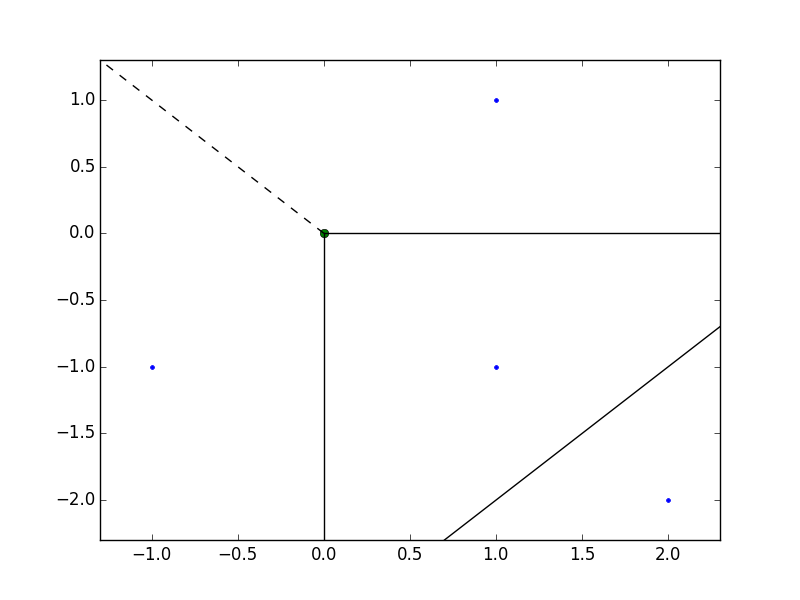
\includegraphics[width=7cm]{Voronoi3a} }}%
	\end{figure}	

The above figure shows the Voronoi map. The above figure was obtained by writing a small piece of code in python. I have included it because I felt me my hand drawn version was not that really pleasing. Either ways I have attached it below:

	\begin{figure}[H]%
		\centering
		\subfloat[Voronoi Map using Euclidean distance (hand drawn)]{{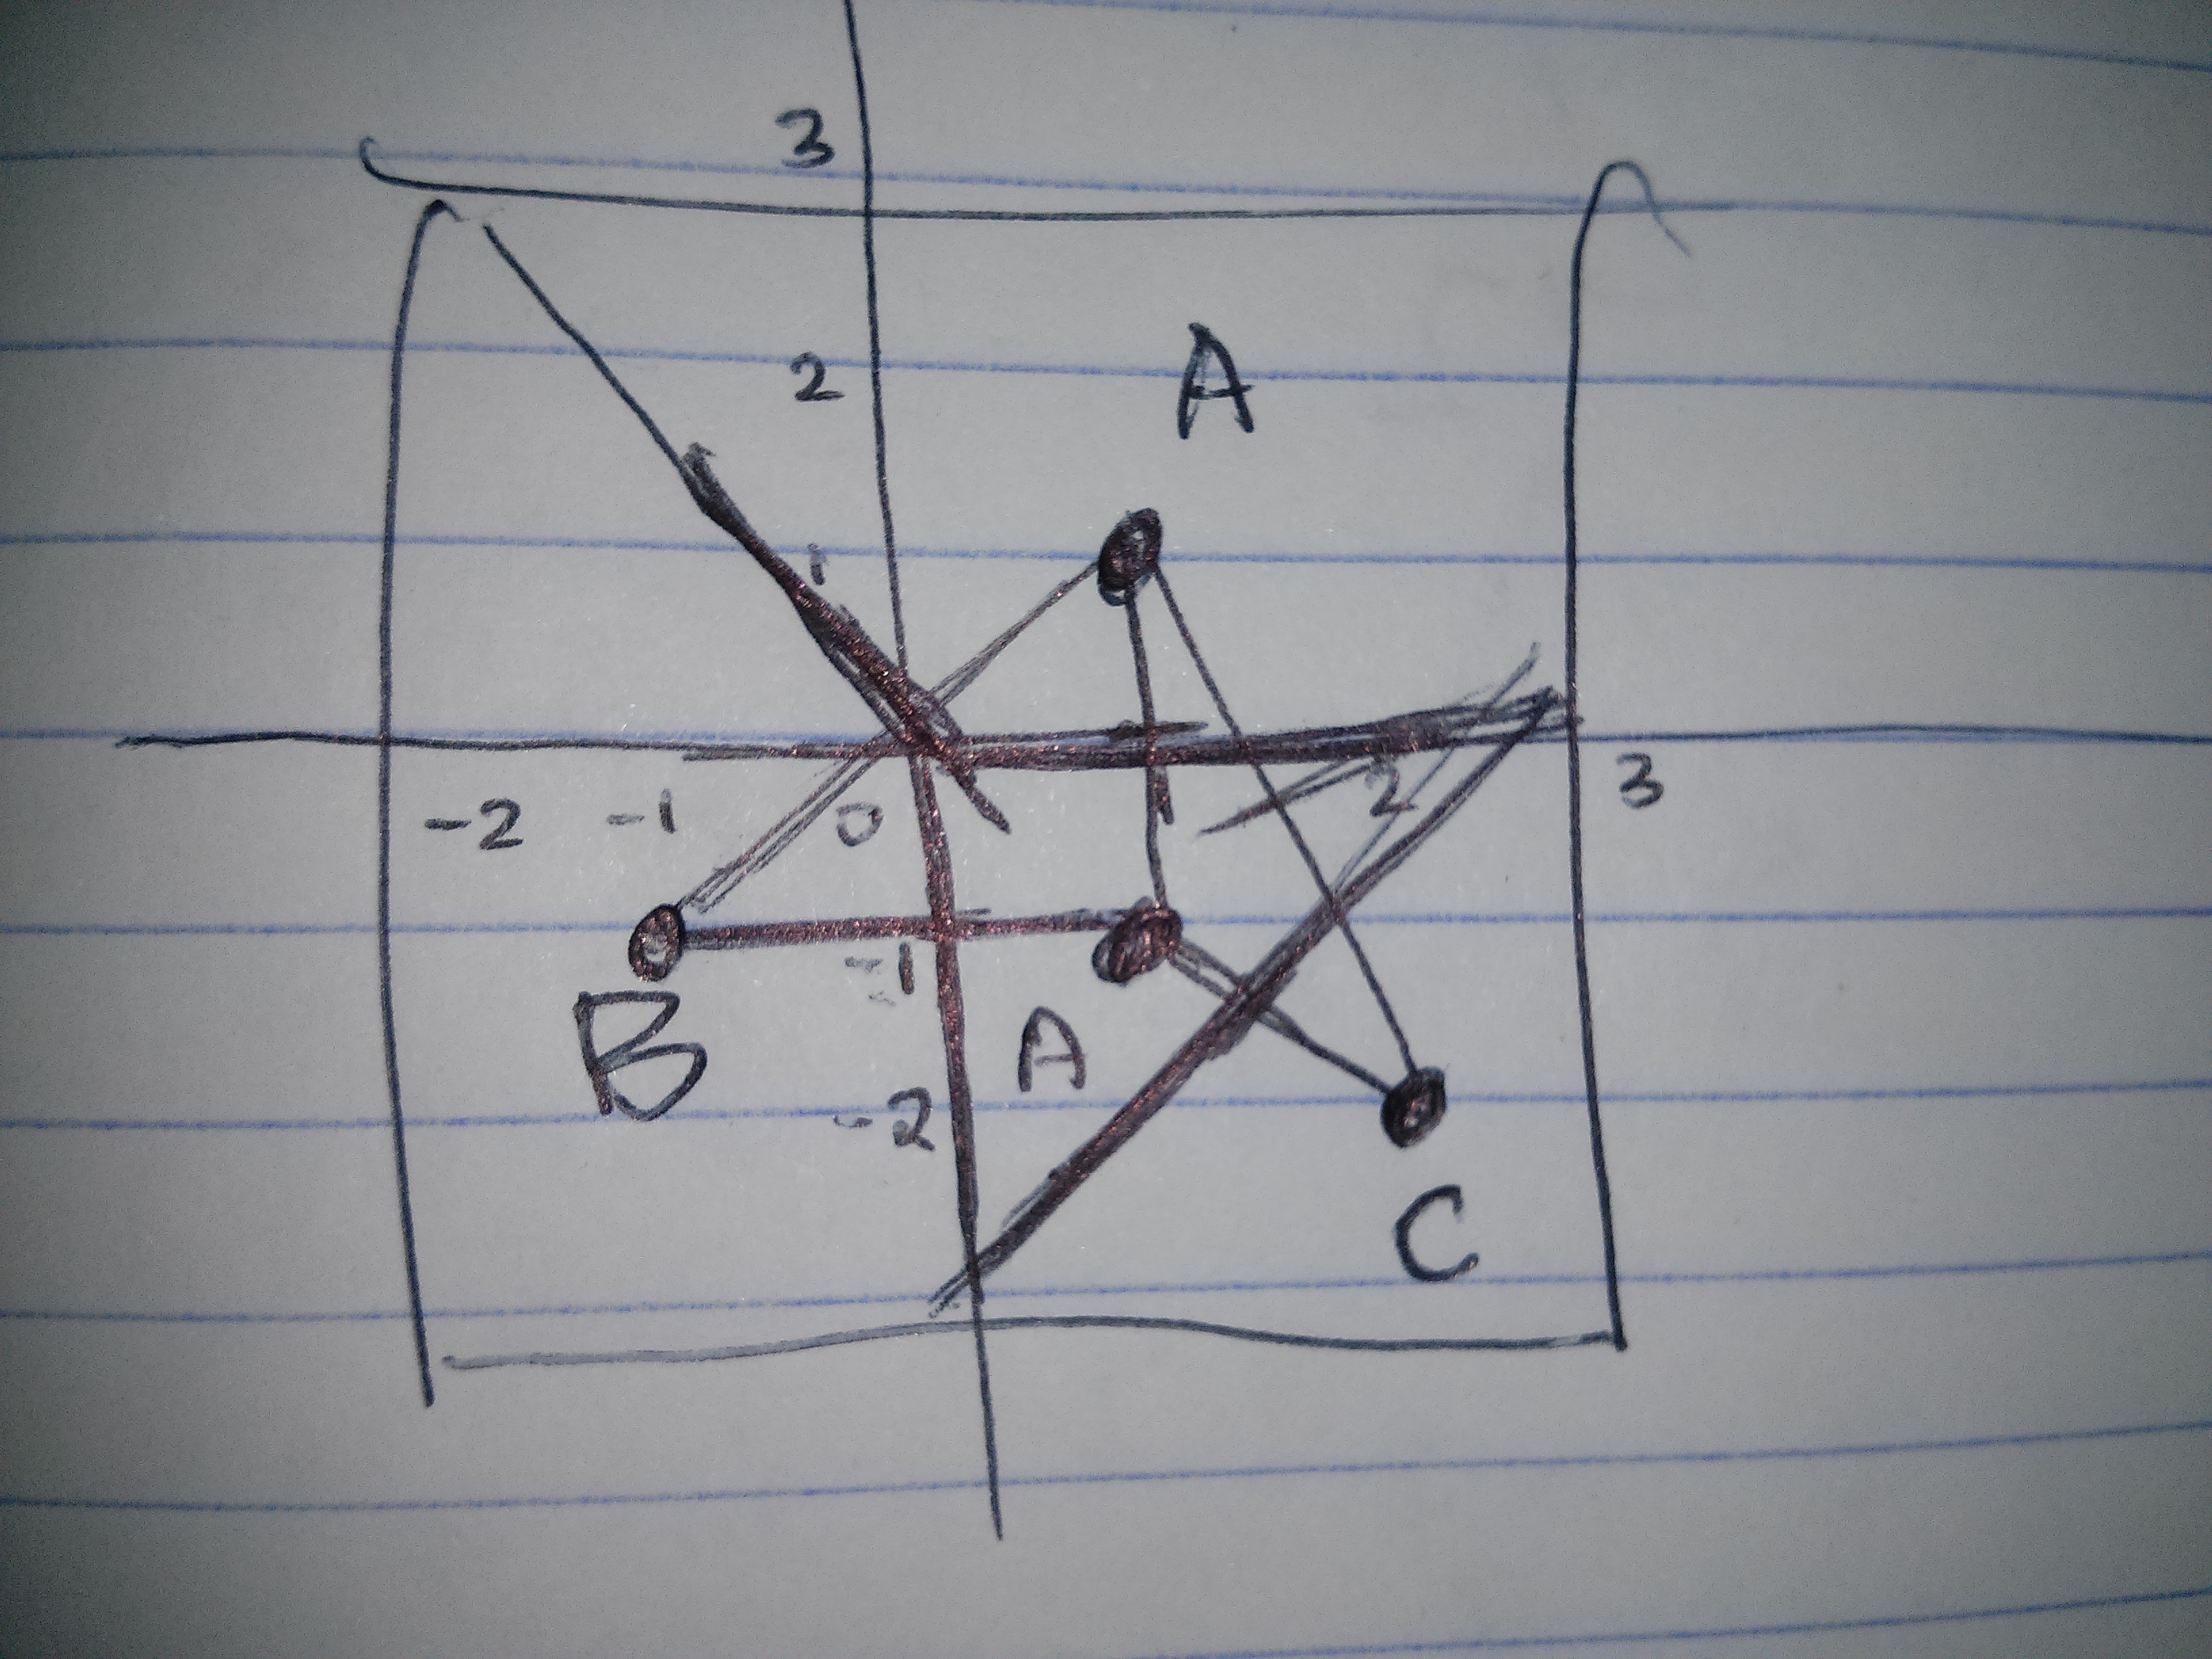
\includegraphics[width=7cm]{3a} }}%
	\end{figure}	
	 
\item[2.] \textbf{[Voronoi Map using Manhattan distance]}	

In this problem we are given with three points A,B,C and are asked to come up with the Voronoi map using Manhattan distance metric.The procedure I followed while drawing the Voronoi diagram is as follows:

1. Plot all the 3 points on paper.\\
2. Measure the Manhattan distances between a point and all its three neighbors \\

For point A(1,1) the distance to its two neighbors are 4,4\\
For point B(-1,-1) the distance to its two neighbors are 4,4\\
For point C(2,-2) the distance to its two neighbors are 4,4\\

3. In this case all the points are equidistant from each other. In fact the points kinda seem to be like three vertices of a triangle and to separate them into Voronoi regions, the intuition is the centroid would divide the points into three different regions. \\
4. Draw the centroid \\
5. Sketch the boundary of the regions and draw the Voronoi map.

	\begin{figure}[H]%
		\centering
		\subfloat[Voronoi Map using Manhattan distance]{{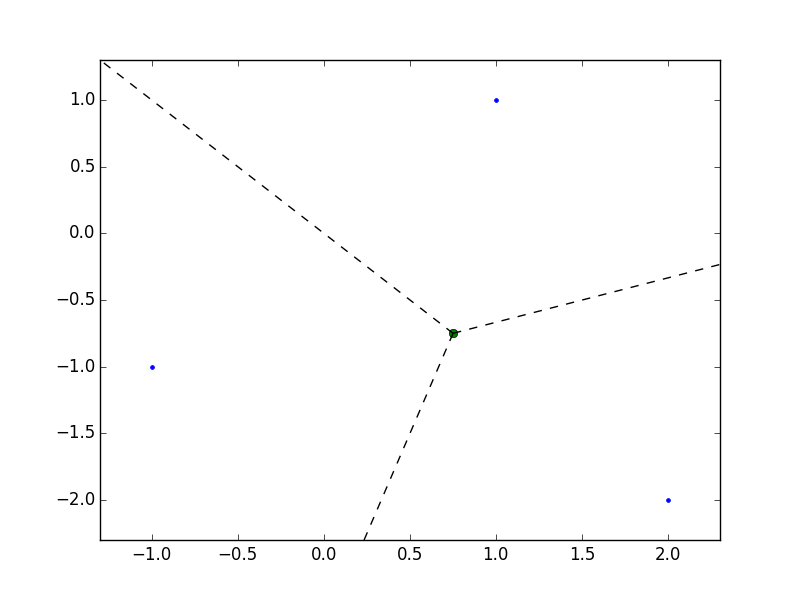
\includegraphics[width=7cm]{Voronoi3b} }}%
	\end{figure}	

I have also included the hand drawn version

\begin{figure}[H]%
	\centering
	\subfloat[Voronoi Map using Manhattan distance]{{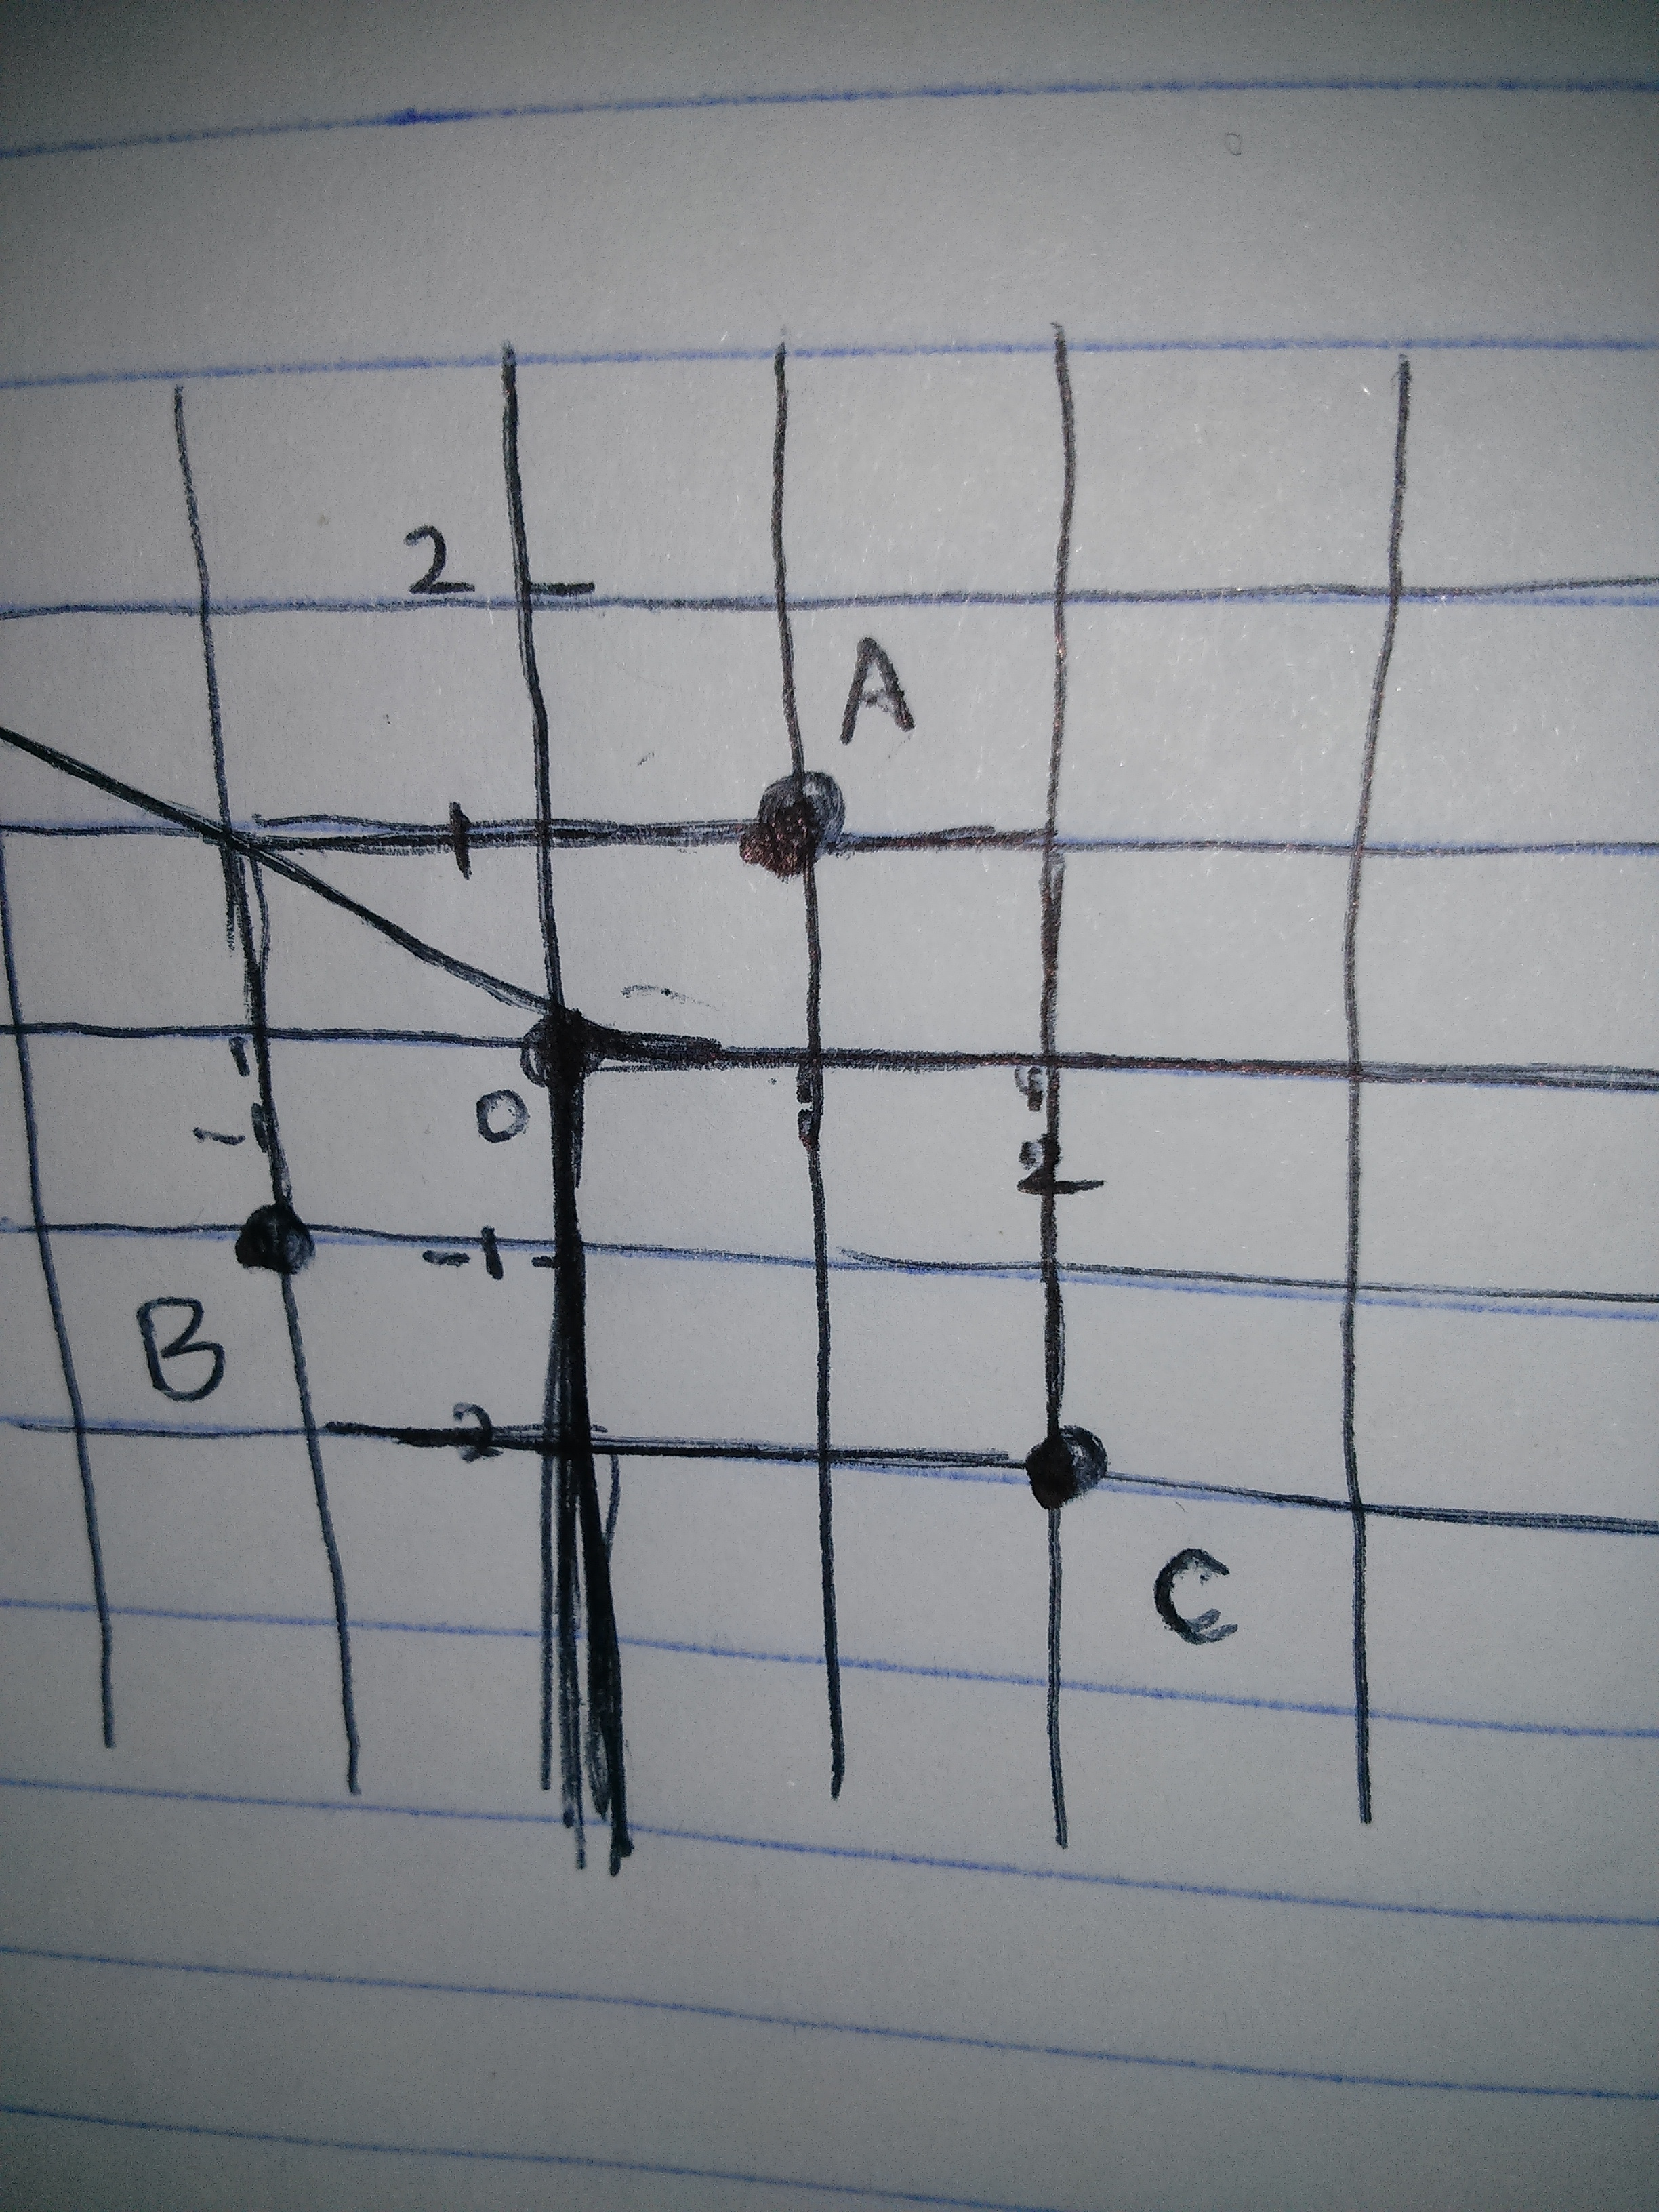
\includegraphics[width=5cm]{3b} }}%
	
\end{figure}

\item[3.] \textbf{[Weighted nearest neighbor]}	

In this problem we are given the formula for determining the score of a point based on the weights of its nearest neighbors where distance decides the value or score. Score is given by the following  formula: \\

$$Score(A) = \sum_{i=1; y_i = A}^M \frac{1}{d({\bf x}_i, {\bf x})}.$$

We are asked to find what would the classification of the test point(4,0) would be with respect to four points specified in the part a of this problem.

$Score(A) =\frac{1}{d(1,1 | 4,0)} + \frac{1}{d(1,-1 | 4,0)}$\\
$Score(A) = \frac{1}{\sqrt{10}} + \frac{1}{\sqrt{10}} $\\
$\boxed{Score(A) = \frac{2}{\sqrt{10}} = 0.634}$\\

$Score(B) =\frac{1}{d(-1,-1 | 4,0)} $\\
$Score(B) =\frac{1}{\sqrt{26}} $\\
$\boxed{Score(B) =0.196}$\\

$Score(C) =\frac{1}{d(2,-2 | 4,0)} $\\
$Score(B) =\frac{1}{2\sqrt{2}} $\\
$\boxed{Score(B) =0.3535}$\\

From the scores we can see thatscore is highest for label A, hence the given testing point should also be given the \textbf{label A}.
The fact that there are two points with label A which are slightly closer to the given test point kind of plays an important role. The distance between the test point and point with label C would be the least in terms of Euclidean distance but the fact that there are more points having label A than C and they are relatively closer to the test point, it gets assigned the label C.

This is one of the potential disadvantages if we could say so as the majority weighting or voting results in the test point getting that label.
	
\end{enumerate}		


\section{The Badges Game (again)}

\begin{enumerate}

\item[1.] \textbf{[Feature functions]}	

For the new badges game, I had come up with four feature functions. They are as follows: \\

\textbf{Feature 1:} If the last letter in the name is between a-m then 0, else 1 \\
\textbf{Feature 2:} If the first letter of the second name is between a-m ,then 1 else 0 \\
\textbf{Feature 3:} If the count of vowels in the name is odd,then 1 else 0 \\
\textbf{Feature 4:} If the string length is even,then 1 else 0 \\ 

For the first name on the list which  is \textbf{ matthias heger}, the feature vector for the name is given by \textbf{(1, 1, 1, 0)}
based on the given feature functions.

\item[2.] \textbf{[Decision Tree data structure]}	

I made use of the following decision tree structure. I had a lot of attributes in the tree which I wanted to make use of in the program. The structure is provided below:

\begin{verbatim}
class Tree:
		def __init__(self, name,parent=None):
			self.parent = parent
			self.children = []
			self.label = None
			self.entropyf1=0
			self.entropyf2=0
			self.name=''
			self.information_gain=0
			self.majority_errorf1=0
			self.majority_errorf2=0
			self.splitFeatureValue = None
			self.splitFeature = None
\end{verbatim}

\item[3.] \textbf{[ID3 Learning Algorithm]}

The decision\_tree.py file which contains my code for the construction of Decision tree takes a txt file or training set as input. It doesthe following in this order:

\begin{enumerate}

\item Defines four feature functions mentioned in part a and derives a feature vector.
\item Calculates the entropy  for the whole dataset
\item Calculate the information gain using entropy as a measure of impurity and determines which is the root attribute
\item Based on the feature selected, it computes the information gain for other features remaning w.r.t to  the feature selected in the previous step of the iteration.
\item Proceeds down until you encounter a node with InformationGain=0 or Entropy=0 or if you have used all the four features.
\item Assigns a label of '+' or '-' to the leaf nodes	

\end{enumerate}

\item[4.] \textbf{[Majority Error based Learning Algorithm]}

This algorithm performs almost as same as the previous one, the only difference being that we make use of Majority Error measure to  calculate the Information Gain.
\begin{enumerate}
	
	\item Defines four feature functions mentioned in part a and derives a feature vector.
	\item Calculates the majority error for the whole dataset
	\item Calculate the information gain using majority error as a measure of impurity and determines which is the root attribute
	
	After this it performs same as the above algorithm in implementing the decision tree. I have both the parts of majority error and entropy measure in the same file and make use of different function calls to see the results.
\end{enumerate}	


\item[5.] \textbf{[K Nearest Neighbor classifier]}

For the K-nearest neighbor the starting point would again be the feature vector created for the names on the set. The Hamming distance is used for finding the distance between two points or examples. The difference in the number of bits between the feature vectors for the two examples is taken into account.

The weighted nearest neighbor formulation which was provided in Question 2 could be made use to determine the score based on the distances and then assign the point a corresponding label.

For odd numbered points the implementation is slightly easier as ties are broken, while for even numbered value of k(2,4) the majority value is used for breaking ties.


\item[6.] \textbf{[Accuracy on testing data]}

The ID3 algorithm was able to predict labels correctly for close to 28 names in the test data. The feature function selected was able to provide 28 correct results out of 94 names.

For K-nearest neighbor I couldn't complete the implementation and so wouldn't be able to provide an exact estimate.

From working out and solving problems and as well as trying out the coding for these algorithms, ID3 algorithm performs or provides much better accuracy than Majority error. On similar lines it should provide better accuracy than K-Nearest neighbors too.

\end{enumerate}

Total time spent on the assignment was spread across few days. I started early after the assignment was out and was working on first problem early. But then due to some own time mismanagement, it took quite some time to finish in the last two days althought I would have hoped to done a even better job by starting earlier. Total time spent was around 30 hours.
	\end{document}
	